%%%%%%齋藤研究室レジュメテンプレート%%%%%%% 2024

\documentclass[a4j]{jsarticle}
\usepackage[utf8]{inputenc}
\usepackage{amsmath,amssymb,amscd,amsthm}
\usepackage{ascmac,fancybox} 
\usepackage{bm}
\usepackage[dvipdfmx]{graphicx}
\usepackage{algorithm}%擬似コードを書く場合
\usepackage{algorithmic}%擬似コードを書く場合
%%%% ↓algotithmic の \REQUIRE と \ENSURE の表記を変更する
\renewcommand{\algorithmicrequire}{\textbf{Input:}}
\renewcommand{\algorithmicensure}{\textbf{Output:}}
%%%% ↑algotithmic の \REQUIRE と \ENSURE の表記を変更する
\def \QED{\hfill $\Box$}%証明終了の記号


%%%%%%%本文%%%%%%% 
\title{レジュメの書き方}
\author{齋藤 翔太}
\date{2024年4月8日}

\begin{document}

\maketitle

%%目的%%
\section*{発表の目的}
プレゼンテーションの基本的な考え方と、それに基づくレジュメの書き方を伝えることが本発表の目的である。


%%目次%%
\tableofcontents

\clearpage

%%本文%%
\section{プレゼンテーションの基本}
レジュメに限らず、どんな媒体を用いるにしても、良いプレゼンテーションを行うためには以下の手順にしたがってストーリーを考える必要がある。

\begin{itembox}[l]{手順1}
目的を明確にする。
\end{itembox}

具体例をあげると以下のようになる。

\begin{description}
\item[本発表]プレゼンテーションの基本的な考え方とレジュメの書き方を伝えること。
\item[学部3年生のゼミ]担当範囲のテキストの内容を理解してもらうこと。担当範囲のうち、自分では理解できなかった部分を正確に伝え、議論すること。
\item[学部4年生のゼミ]自分の研究の進捗を正確に報告し、今後の研究の進め方についてのアドバイスをもらうこと。
\end{description}

\begin{itembox}[l]{手順2}
聴衆は誰か考える。
\end{itembox}

プレゼンテーションの良し悪しはそのときの聴衆にとってわかりやすかったかどうかで決まる。発表の目的と聴衆の前提知識を突き合わせることで、何をどのような順番でどんな側面から説明すべきかが決まる。具体例をあげると以下のようになる。

\begin{description}
\item[学部3年生のゼミ] 齋藤研究室の学生全体。
\item[4年生の卒論発表会] 情報学部の他の教員。
\end{description}

\begin{itembox}[l]{手順3}
発表時間に応じて盛り込む内容を決定する。
\end{itembox}

発表時間とプレゼンテーションの目的を達成するのに重要なものを考慮して、発表に盛り込む。具体例は以下のようになる。

\begin{description}
\item[本発表]発表時間は15分程度。優先度は高い順に、プレゼンテーションの基本、レジュメを書くときのポイント、発表内容ごとの具体例。
\end{description}

\section{レジュメを書くときのポイント}
レジュメを作成するときは、特に以下の点に注意する。
他の形式的な注意点は付録にまとめてあるので、それらも参照のこと。

\begin{itemize}
\item 正確に書く
\begin{itemize}
\item 式で書く
\item 擬似コードで書く
\item 変数がとりうる値の範囲を書く(例えば、「○○を$x$とおく」よりも「○○を$x \in \mathbb{R}$とおく」等と書く)
\item 写像(関数)なら始集合と終集合を書く(例えば、「関数$f$」よりも「関数$f : \mathbb{R} \to \mathbb{R}$」等と書く)
\item $\sum_{i,j}x_i y_j$より$\sum_{i=1}^n \sum_{j=1}^m x_i y_j$等と書く
\item 解釈の仕方が1通りしかないような文章にする
\end{itemize}

\item 直観的にわかるように書く
\begin{itemize}
\item 図で書く
\item フローチャートを使う
\item 式で書く
\item 箇条書きで書く
\item 擬似コードで書く
\item 重要なところほど目立たせる
\begin{itemize}
\item 枠囲みを使う
\item 太字にする
\item 下線を引く
\end{itemize}
\item 本質的でない議論を脚注\footnote{これが脚注である。}や付録に回す
\end{itemize}

\item 具体例を書く
\begin{itemize}
\item 新たに定義された概念について、変数に値を代入してイメージをつかむ
\item 変数に値を代入して定理を確かめる
\item 変数に値を代入したもとで、アルゴリズムの挙動を追う
\end{itemize}

\item わからなかったところを明確に書く
\begin{itemize}
\item わかったふりをしない
\item 「式(a)から式(b)への変形がわからなかった」等、具体的であるほど良い
\end{itemize}
\end{itemize}

\section{発表内容ごとの具体例}

\subsection{定理とその証明の書き方}
定理とその証明を述べるという発表も多い。
その際には以下に注意する。
\begin{itembox}[l]{定理とその証明の書き方}
\begin{itemize}
\item 定理は枠囲みを使って強調する
\item 定理の主張そのものが複雑な場合には、その定性的な意味を端的に述べる
\item 証明が長い場合には、あらかじめその証明の構成をフローチャート等を用いて説明する
\end{itemize}
\end{itembox}

\subsubsection{定理とその証明の書き方の具体例}

\begin{itembox}[l]{定理(相互情報量とエントロピーの関係)}
確率変数$X$と$Y$について、以下の関係式が成り立つ。
\begin{align}
I(X; Y) = H(X) - H(X|Y) \label{relationship}
\end{align}
\end{itembox}

式\eqref{relationship}の左辺$I(X; Y)$は$Y$を知ったときに$X$に関して得られる情報量を表し、式\eqref{relationship}の右辺は$X$の不確かさ$H(X)$から$Y$を知ったとしても残っている$X$の不確かさ$H(X|Y)$を引き算したものを表している。すなわち、相互情報量は不確かさの減少量で表現できることを表している。

\medskip

証明:
相互情報量$I(X; Y)$を次のように変形する。
\begin{align}
I(X; Y) 
&\overset{(a)}{=} \sum_{x \in {\cal X}} \sum_{y \in {\cal Y}} P_{XY} (x,y) \log_2 \frac{P_{XY} (x,y)}{P_{X}(x)P_{Y}(y)} \\
&= \sum_{x \in {\cal X}} \sum_{y \in {\cal Y}} P_{XY} (x,y) \log_2 \frac{P_{X|Y} (x|y)}{P_{X}(x)} \\
&= - \sum_{x \in {\cal X}} \sum_{y \in {\cal Y}} P_{XY} (x,y) \log_2 P_{X} (x) + \sum_{x \in {\cal X}} \sum_{y \in {\cal Y}} P_{XY} (x,y) \log_2 P_{X|Y} (x|y) \\
&= - \sum_{x \in {\cal X}} P_{X} (x) \log_2 P_{X} (x) - \left( -\sum_{x \in {\cal X}} \sum_{y \in {\cal Y}} P_{XY} (x,y) \log_2 P_{X|Y} (x|y) \right) \\
&\overset{(b)}{=} H(X) - H(X | Y)
\end{align}
ここで、$(a)$は相互情報量の定義、$(b)$はエントロピーと条件付きエントロピーの定義による。
ゆえに、$I(X; Y) = H(X) - H(X|Y)$が成り立つ。
\QED

\subsection{アルゴリズムの書き方}
アルゴリズムを記述するときのポイントは以下の通りである。

\begin{itembox}[l]{アルゴリズムの書き方}
\begin{itemize}
\item 入力、出力、処理をすべて明記する
\item 擬似コードを使って書くとなお良い
\item 具体例による説明を添える
\end{itemize}
\end{itembox}

\subsubsection{アルゴリズムの書き方の具体例}

消失訂正sum-product復号法を例に説明すると以下のようになる。消失訂正sum-product復号法は、消失通信路上でLDPC符号を復号する際によく用いられる復号法である。以下のアルゴリズムやその具体例の説明は\cite{wadayama}を参考にしたものである。

\begin{description}
\item[初期化]
受信語$\bm y \in \{ 0, 1, \mathrm{?}\}^n$の各成分$y_i$値に応じて、対応する変数ノード$v_i \in V$の変数ノード値$n_{v_i}$を以下のように初期化する。
\begin{align}
n_{v_i} &= 
\begin{cases}
1, & y_i = 0\\
-1, & y_i = 1\\
0, & y_i = \mathrm{?}
\end{cases}
\end{align}

\item[変数ノード処理]
変数ノード$v_i \in V$から隣接するチェックノード$c_j \in \mathcal{N}(v_i)$へ送られるメッセージ$m_{v_i \to c_j}$は以下のようになる。
\begin{align}
m_{v_i \to c_j} = n_{v_i}
\end{align}
\item[チェックノード処理]
チェックノード$c_j \in C$から隣接する変数ノード$v_i \in \mathcal{N}(c_j)$へ送られるメッセージ$m_{c_j \to v_i}$は以下のようになる。
\begin{align}
m_{c_j \to v_i} = \prod_{v_k \in \mathcal{N}(c_j) \backslash \{ v_i \}} m_{v_k \to c_j}
\end{align}
\item[変数ノード値の更新]
変数ノード値$n_{v_i}$は以下のように更新される。
\begin{itemize}
\item 隣接するチェックノード$c_j \in \mathcal{N}(v_i)$から送られるメッセージ$m_{c_j \to v_i}$と変数ノード値$n_{v_i}$が全て$0$のとき、変数ノード値は$n_{v_i} = 0$とする。
\item 隣接するチェックノード$c_j \in \mathcal{N}(v_i)$から送られるメッセージ$m_{c_j \to v_i}$と変数ノード値$n_{v_i}$に1つでも$0$でない値が含まれる場合、その値を変数ノード値$n_{v_i}$とする。
\end{itemize}
\item[$\hat{\bm x}$の計算]
変数ノード値$n_{v_i}$をもとに、復号語$\hat{\bm x} \in \{ 0, 1\}^n$の各成分$x_i$を以下で決定する。
\begin{align}
x_i = 
\begin{cases}
0, & n_{v_i} = 1\\
1, & n_{v_i} = -1
\end{cases}
\end{align}
\end{description}

アルゴリズムを疑似コードで記述すると、次のページようにまとめられる。
また、具体例を用いて各処理を説明すると以下の図\ref{erasure_collecting}のようになる。

%%消失訂正sum-product復号法の擬似コード%%
\begin{algorithm}
\caption{消失訂正sum-product復号法}
\label{alg1}
\begin{algorithmic}
\REQUIRE 受信語$\bm y \in \{ 0, 1, \mathrm{?}\}$,タナーグラフ$G(V \cup C, E)$
\ENSURE 復号語$\hat{\bm x} \in \{ 0, 1\}^n$またはerror
\FORALL[初期化]{$v_i \in V, c_j \in \mathcal{N}(v_i)$}
	\STATE $n_{v_i}$を初期化
\ENDFOR
\WHILE{変数ノード値が更新され続ける限り}
	\FORALL[変数ノード処理]{$v_i \in V, c_j \in \mathcal{N}(v_i)$}
		\STATE $m_{v_i \to c_j}$を更新
	\ENDFOR
	\FORALL[チェックノード処理]{$c_j \in C, v_i \in \mathcal{N}(c_j)$}
		\STATE $m_{c_j \to v_i}$を更新
	\ENDFOR
	\FORALL[変数ノード値の更新]{$v_i \in V$}
		\STATE $n_{v_i}$を更新
	\ENDFOR
\ENDWHILE
\FORALL{$v_i \in V$}
	\IF{$n_{v_i} = 0$}
		\RETURN error
	\ENDIF
	\STATE $\hat{x}_i$を計算
\ENDFOR
\RETURN $\bm \hat{\bm x}$
\end{algorithmic}
\end{algorithm}

%%消失訂正sum-product復号法の図%%
\begin{figure} [htbp]
\centering
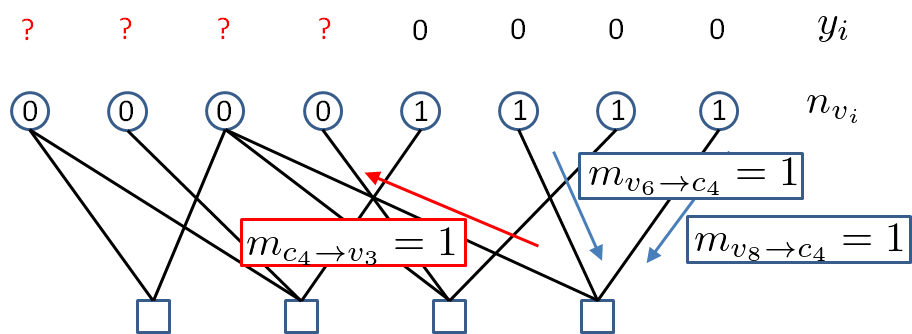
\includegraphics[width=10cm]{sumproduct.png}
\caption{消失訂正sum-product復号法}
\label{erasure_collecting}
\end{figure}

\section{\LaTeX について}
この資料は、\LaTeX を用いて作成した。これまでに\LaTeX を使ったことがない学生は、Overleafを用いて使うとよい。Overleafの設定については、Slackにアップロードした資料を参照のこと。

理工学の論文は\LaTeX を用いて書くことが多いので、徐々に使えるようにしていくこと。また、この資料の\LaTeX ソースコードをSlackにアップロードしておくので、自分でレジュメを作成する際のテンプレートファイルとして使うとよい。

\section{まとめ}
プレゼンテーションの基本的な考え方と、それに基づくレジュメの書き方を説明した。

%%参考文献%%
%\newpage
\begin{thebibliography}{99}
\bibitem{wadayama}和田山正,誤り訂正技術の基礎,森北出版,2010.
\end{thebibliography}

%%付録(目次に反映)%%
\clearpage
\addcontentsline{toc}{section}{付録} %bookのときはsection->chapter
\appendix
\section{形式的な注意}
\begin{itemize}
\item ページ番号を振る
\item 式番号を振る
\item 図、表番号を振る
\item 代表的な構成は
\begin{enumerate}
\item タイトル
\item 発表の目的
\item 目次
\item その発表の内容
\item まとめと(もしあるなら)今後の課題
\item 参考文献
\item 付録
\end{enumerate}
\end{itemize}

\section{参考文献の書き方}\label{reference}
発表の際に参考にした文献があれば参考文献として書いておく。形式は以下の通り。
\begin{description}
\item[書籍]\mbox{}\\
著者,タイトル,出版社,出版年.
\item[論文]\mbox{}\\
著者,``タイトル,'' 論文誌名,巻数,号数,該当ページ,発行年.
\end{description}
細かい注意点は以下の通り。
\begin{itemize}
\item 日本語の文献では「,」や「.」は全角。英語の文献では半角+半角スペース。
\item 該当ページの入力はpp. 00--00とする。間のハイフンは2回続けて入力する
\item 和書の場合は巻末、洋書の場合はタイトルページの裏側にある奥付を読めば出版社や出版年がわかる。
\end{itemize}

\end{document}
